\chapter{Evaluation}
\label{eval}

This chapter provides an insight into the data collected from the questionnaires and \methodname system logs while also explaining results derived from statistical tests. The chapter is structured as follows: \S\ref{sec:eval-experiment} gives an overview of the hardware used. \S\ref{sec:eval-demographic} provides an over of the demographic background for the sampled participants. \S\ref{sec:eval-distTests} covers test which check the data sets distribution moving on to compare the distribution across the feedback group and control group. \S\ref{sec:eval-feedbackSysResults} goes through determining any difference between the two groups which might have been cuased by the introduction of the feedback system. \S\ref{sec:eval-usersFeedback} covers the participants impressions on the experiment and finally conclusive results from this study are presented in \S\ref{sec:eval-Discussion} 

\section{Experiment Setup}
\label{sec:eval-experiment}

The experiment has been carried out using the methods specified in chapter \ref{chp:methodology}. The hardware includes a 32inch LCD Samsung monitor capable of outputting stereo audio and running Assetto Corsa at the resolution of 1920*1080. Assetto Corsa and \methodname run on a PC with an i7 cpu, GTX 980 video, X RAM card and Windows 10 operation system.

\emph{not sure about the PC specs, could you confirm them ? I will add a ref to the product site afterwards}

\begin{figure}
	\centering
	\begin{minipage}{0.45\textwidth}
		\centering
		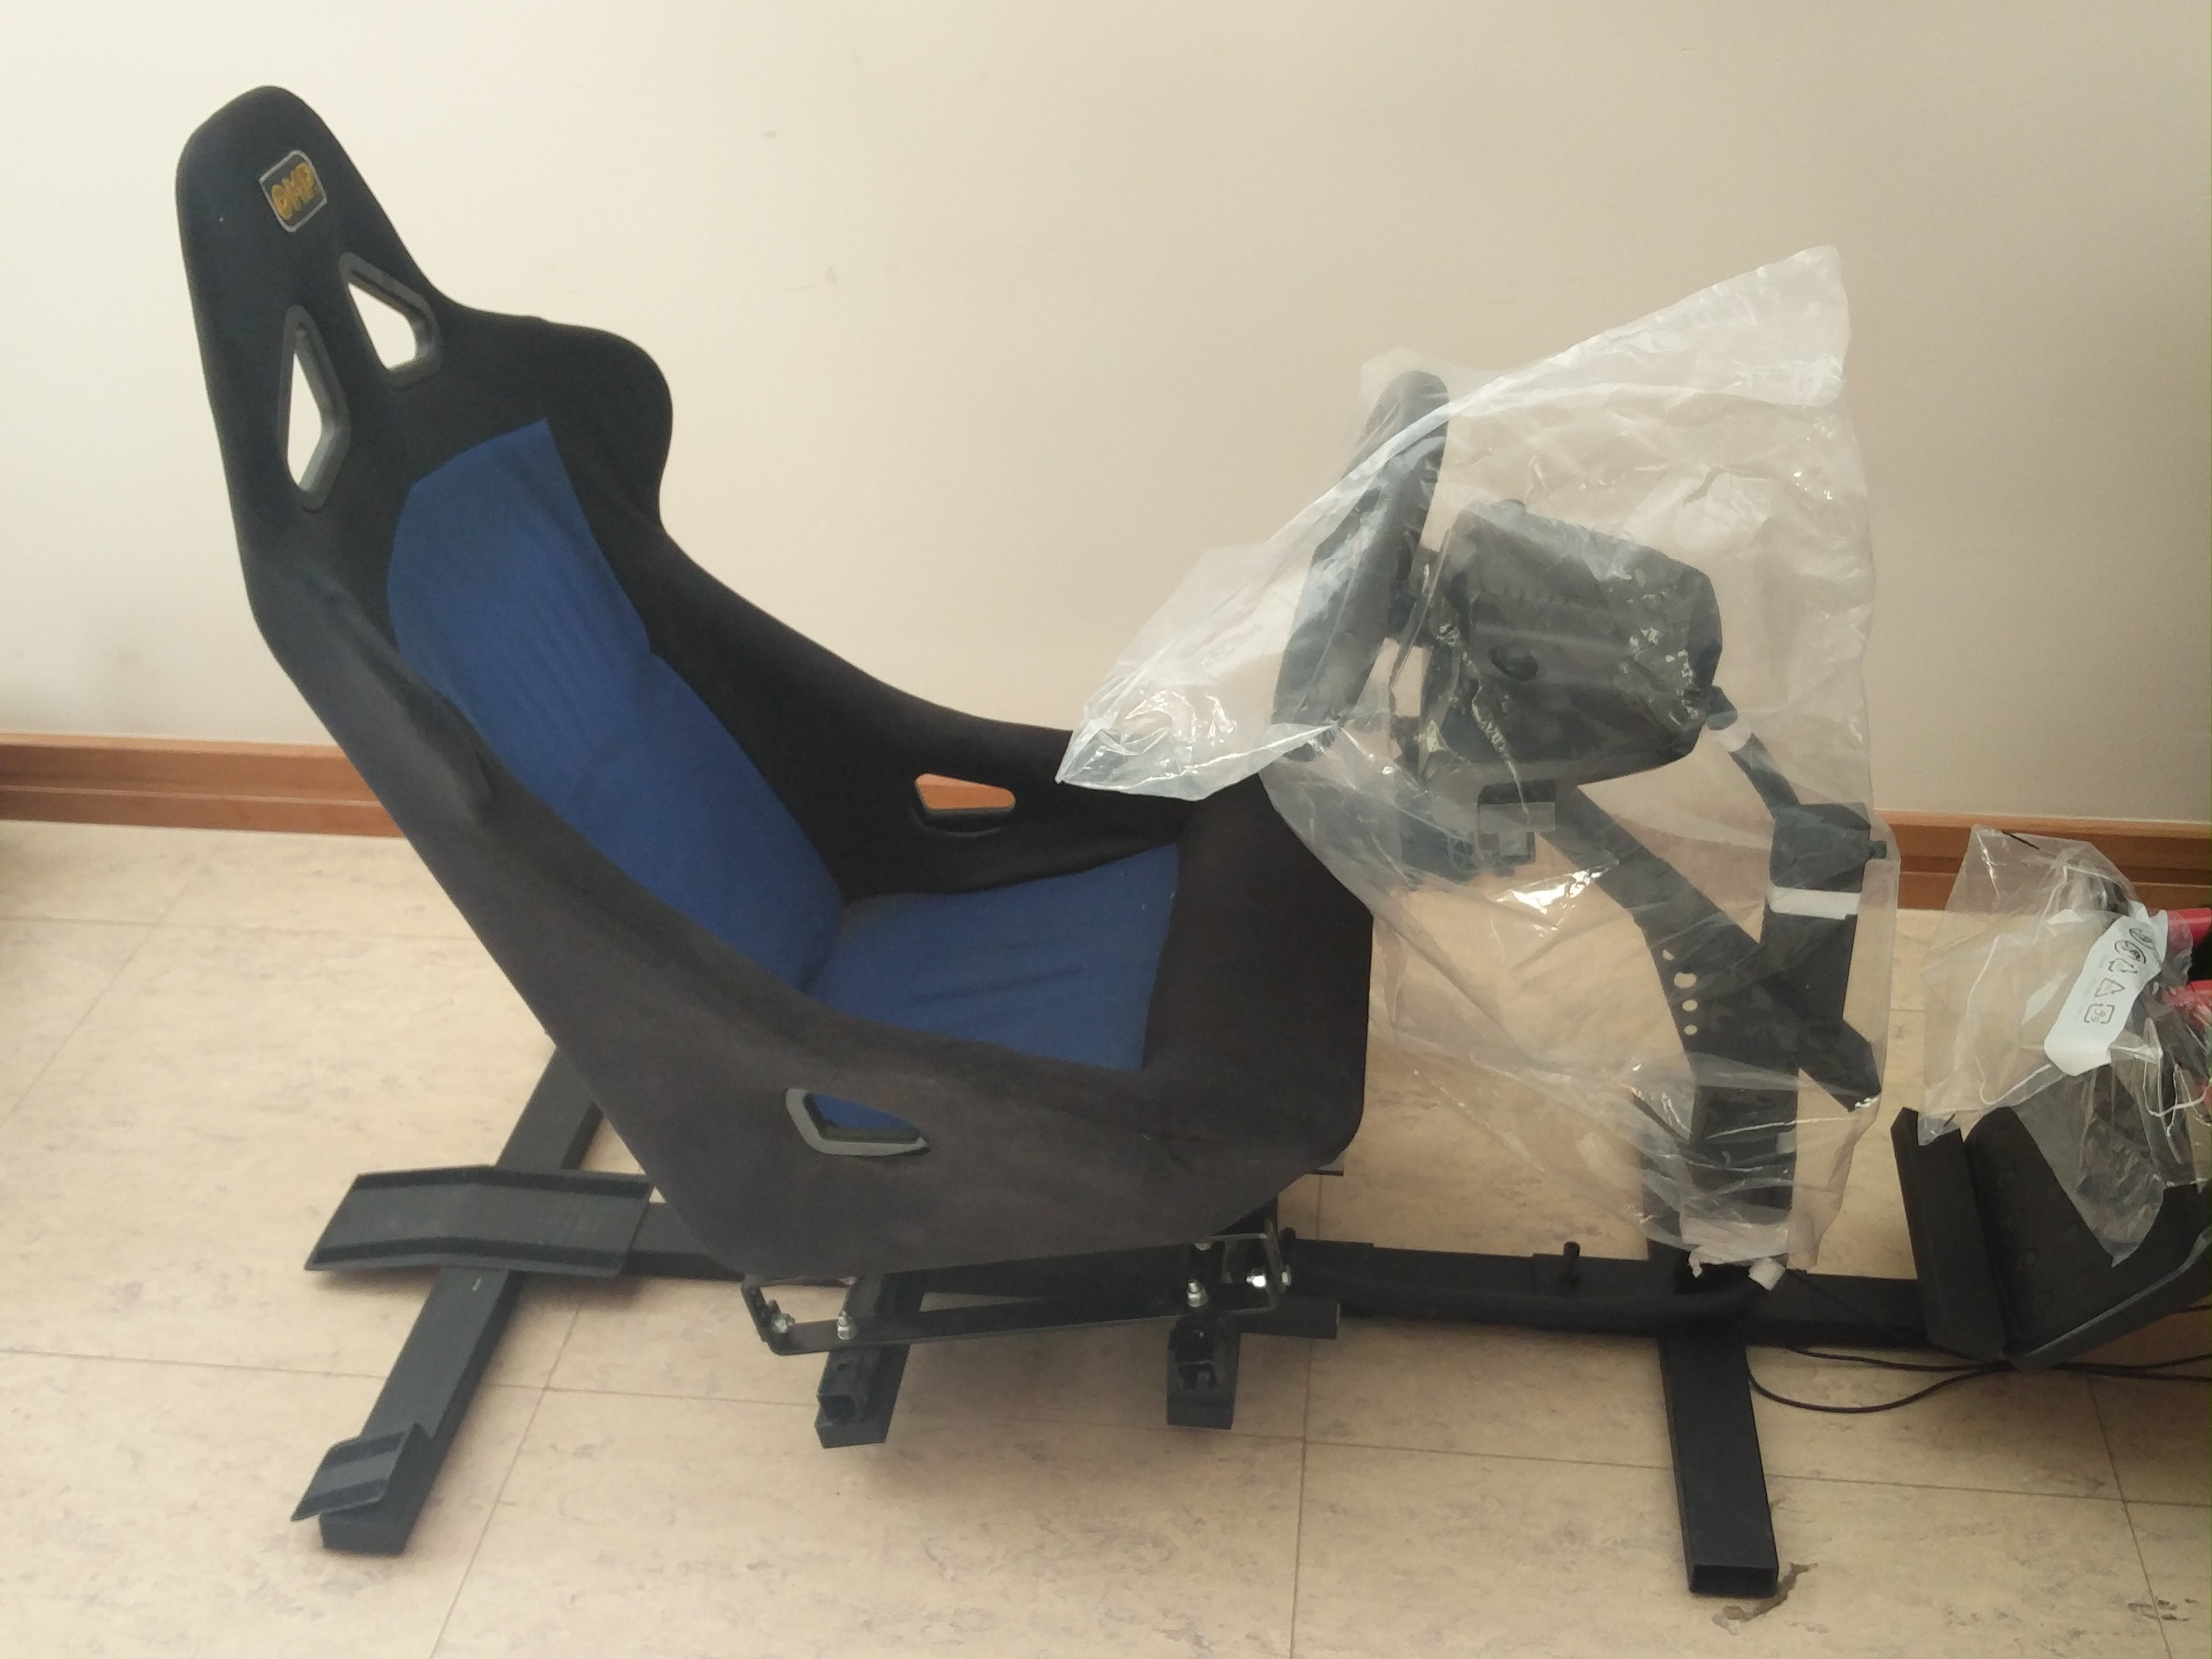
\includegraphics[width=\textwidth]{images/RacingRig}
	\end{minipage}\hfill
	\begin{minipage}{0.45\textwidth}
		\centering
		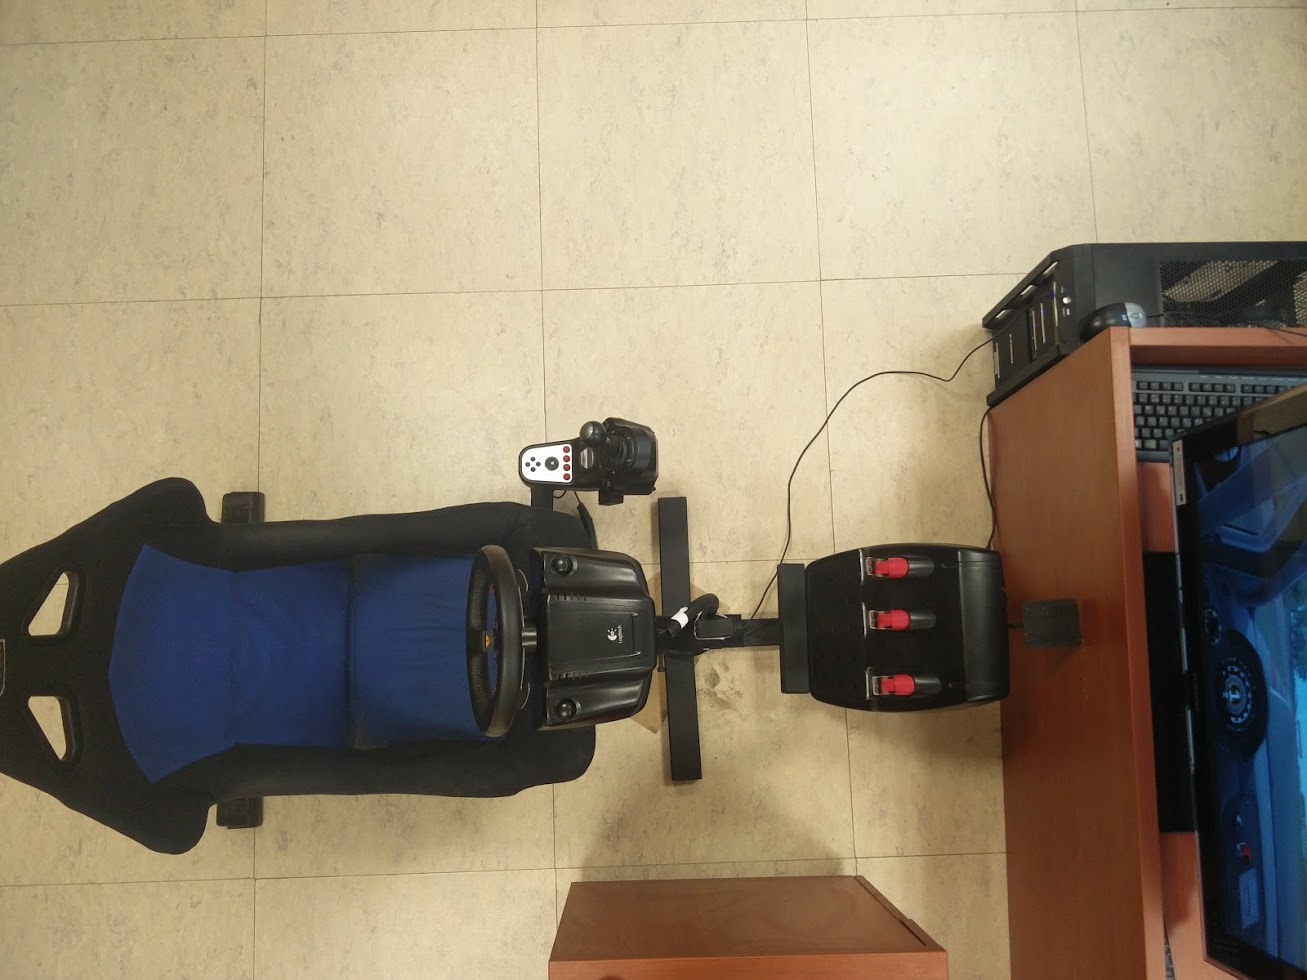
\includegraphics[width=\textwidth]{images/RacingRig2}
	\end{minipage}
	\caption[Side and top view of the racing rig]{Side and top view of the racing rig}
	\label{sec:eval-simRacingRig}
\end{figure}

\section{Sample Demographic}
\label{sec:eval-demographic}

The following demographic data was drawn out from the pre study survey. Participant's were mostly in their early twenties and mostly males (see Figure \ref{fig:chart-genderage}). Out of 27 participants, 2 didn't have a driving license and 25 had a driving license with most of them having been driving for a year (see Figure \ref{fig:chart-licenseddriversexperience}). Furthermore 22 participants identified them self as playing videos games (see Figure \ref{fig:chart-playVideoGames}), from which 18 participants stated they have played racing video games. The majority of participants who plays racing games identified them self as playing mostly arcade sim racing games, while only 3 play sim racing games (see Figure \ref{fig:chart-gamesGenrePlayed}). Out of the 27 participants, 7 participants have previously used a racing rig (see Figure \ref{fig:chart-usedARacingRig}). The groups have been split as follows, 13 in the control group and 14 in the feedback group.
%didn't add another pie chart as I feel they aren't adding much, but if you think it would help, I can add it

\section{Distribution Tests}
\label{sec:eval-distTests}

Histograms for the datasets used during tests which are found in this section are reproduce at Figure \ref{hist-1}

\begin{figure}[!htb]
	\centering
	\includegraphics[width=\textwidth]{charts/laptimes.png}
	\caption[Lap times vs session, clustered by group]{Blue : Control Group, Green : Feedback group \\ Lap times vs session, clustered by group}
	\label{fig:chart-laptimes}
\end{figure}

From the lap times box plot (see Figure \ref{fig:chart-laptimes}), one can notice a trend in which lap times improve the more time participants use the rig, irrespective of the group assignment. It's worth pointing out the median of the feedback group is lower than the control group's median, except during the last session in which the medians are close to each other. Moreover the participants in the feedback group seem to be less consistent in their lap times as the box plot whiskers and quartiles are further spread out than the ones from the control group.

The Shapiro-Wilk Test for normality has been carried out on both the feedback group and control group. The dataset covered the lap times during the first session. The results are shown in Table \ref{table:shapiroWilk}. The p-value for the control group was found to be 0.013 and the feedback group had a p-value of 0.02. With both having a p-value lower than 0.05, the Shapiro-Wilk Test alternative hypothesis is accepted which states the samples do not come from a normally distributed dataset.

\begin{table}[]
	\centering
	\begin{tabular}{ll|rrr|}
		\cline{3-5}
		&                         & \multicolumn{3}{c|}{\textbf{Shapiro-Wilk}}                          \\ \cline{2-2}
		\multicolumn{1}{l|}{\textbf{}}                          & \textbf{Group}          & \textbf{Statistic}        & \textbf{df}             & \textbf{Sig.} \\ \hline
		\multicolumn{1}{|c|}{\multirow{2}{*}{\textbf{LapTime}}} & \textbf{Control Group}  & \multicolumn{1}{r|}{.955} & \multicolumn{1}{r|}{70} & .013          \\ \cline{2-5} 
		\multicolumn{1}{|c|}{}                                  & \textbf{Feedback Group} & \multicolumn{1}{r|}{.963} & \multicolumn{1}{r|}{81} & .020          \\ \hline
	\end{tabular}
	\caption[Shapiro Wilk Test results]{Shapiro Wilk Test results}
	\label{table:shapiroWilk}
\end{table}

The same dataset as used for the Shapiro-Wilk Test was used to run the Kolmogorov-Smirnov Test. The results are shown in Figure \ref{fig:chart-KolmogorowSmimov}. With a significance level of 0.05 and a result having a p-value of 0.360 the null hypothesis is accepted. The groups share the same distribution.

\begin{figure}[!htb]
	\centering
	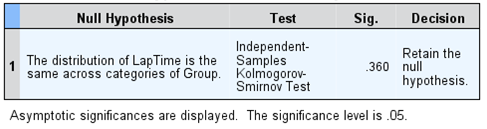
\includegraphics[width=\textwidth]{images/KolmogorowSmimov.png}
	\caption[Kolmogorow Smimov Test]{Kolmogorow Smimov test result}
	\label{fig:chart-KolmogorowSmimov}
\end{figure}

\section{Experiments Results}
\label{sec:eval-ExperimentsResults}

Histograms for the datasets used during tests which are found in this section are reproduce at Figure \ref{hist-1}, Figure \ref{hist-2}, Figure \ref{hist-3} and Figure \ref{hist-4}

Having established both groups' lap times share the same distribution during the first session, the Mann-Whitney Test is used to determine if any differences between the groups exist before \methodname is introduced to the feedback group. The results of the test are shown in Table \ref{table:Mann-Whitney}. These show a p-value of 0.057 with a confidence interval of 0.95 resulting in no statistical difference between the groups at the start of the sessions as the p-value is greater than 0.05, accepting the alternative hypothesis.

\begin{table}[!htb]
	\centering
	\begin{tabular}{|ll|r|rr|r|}
		\hline
		& Group    & \multicolumn{1}{l|}{N} & \multicolumn{1}{l|}{Mean Rank} & \multicolumn{1}{l|}{Sum of Ranks} & \multicolumn{1}{l|}{Asymp. Sig. (2-tailed)} \\ \hline
		\multicolumn{1}{|l|}{\multirow{3}{*}{LapTime}} & Control  & 70                     & \multicolumn{1}{r|}{83.29}     & 5830.50                           &                                             \\ \cline{2-5}
		\multicolumn{1}{|l|}{}                         & Feedback & 81                     & \multicolumn{1}{r|}{69.70}     & 5645.50                           &                                             \\ \cline{2-5}
		\multicolumn{1}{|l|}{}                         & Total    & 151                    &                                &                                   & .057                                        \\ \hline
	\end{tabular}
	\caption[Mann-Whitney Test results]{Mann-Whitney Test results}
	\label{table:Mann-Whitney}
\end{table}

The Mann-Whitney Test was carried out on the second, third and forth session, all tests using a condidence interval of 0.95. The results for these tests are shown in Table \ref{table:Mann-Whitney-Sessions}. The second session has a p-value of 0.054, and the forth session has a p-value of 0.539, both values being above the significance level of 0.05, resulting in the alternative hypothesis being accepted for these sessions. The third session has a p-value of 0.29, being below the significance results in accepting the null hypothesis.

% I am not entrely sure if h0 and h1 are correct, I am sure that p-value > 0.05 = no differnce, p-value < 0.05 = differnce. I might have switched the convetionaly way of defining h0 and h1, Any idea if this is the case ? If I understand this [http://www.statstutor.ac.uk/resources/uploaded/mannwhitney.pdf] correctly, I have switched them

\begin{table}[]
	\centering
	\begin{tabular}{|l|l|l|l|}
		\hline
		& \multicolumn{3}{c|}{LapTime}            \\ \cline{2-4} 
		& 2nd Session & 3rd Session & 4th Session \\ \hline
		Asymp. Sig. (2-tailed) & .054        & .029        & .539        \\ \hline
	\end{tabular}\\
	Grouping Variable : Group
	\caption[Mann-Whitney Test for last three Sessions]{Mann-Whitney test result for the last three sessions}
	\label{table:Mann-Whitney-Sessions}
\end{table}

\section{Participant Feedback}
\label{sec:eval-usersFeedback}
Participants reported an overall good experience, the rig setup was found to be realistic and easy to use (see Figure \ref{fig:chart-feedbacksystemfeedback}. An overwhelming majority of the participants reported having issues mastering the second and third corners (refereed to as the s-bend). Participants also reported the car and track choice to be adequate. When the feedback group was asked about the \methodname, they reported it to be intelligible, accurate, helpful and somewhat easy to apply the feedback given. Lastly, when asked about if they found the feedback to be intrusive, possible distracting them, out of 15, 10 reported to not finding it intrusive (see Figure \ref{fig:chart-intrusivefeedback}).

\begin{figure}[!htb]
	\centering
	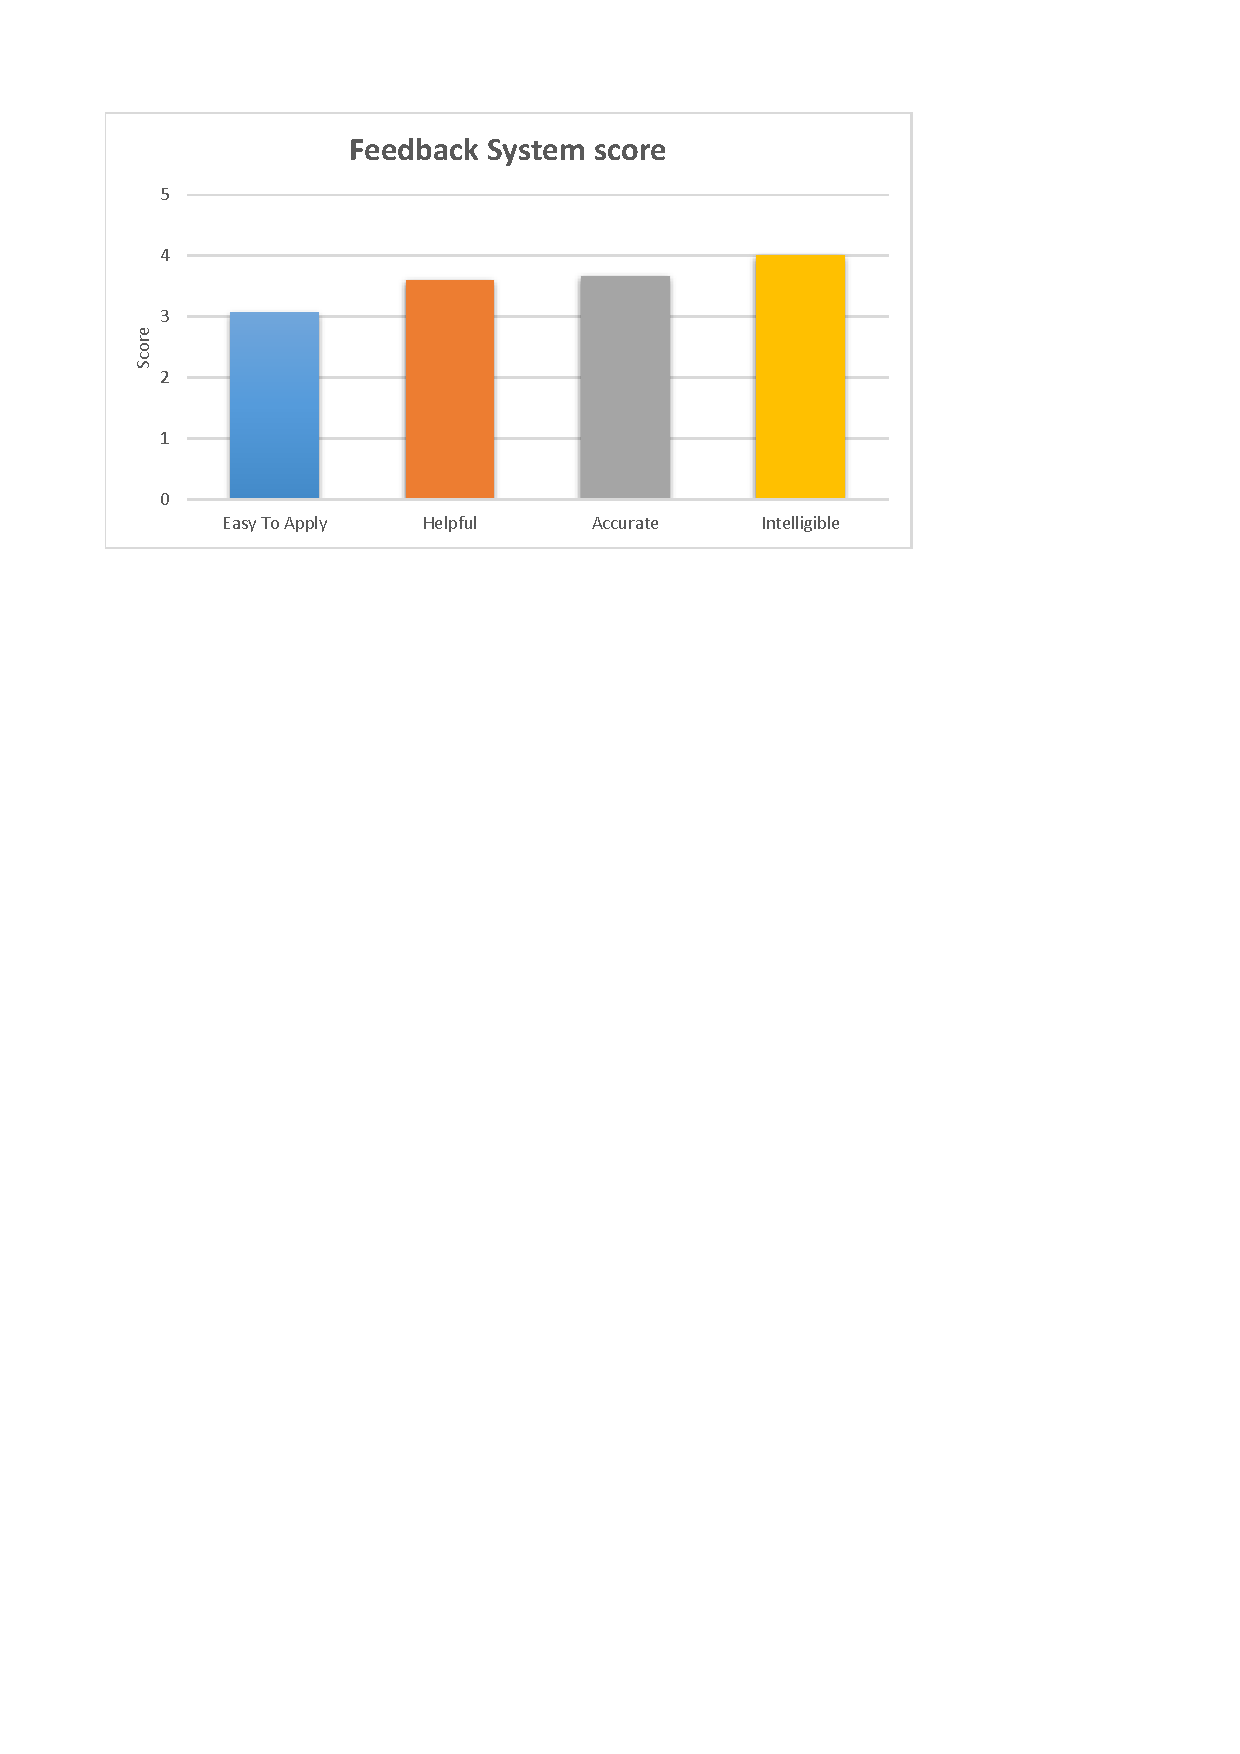
\includegraphics[width=\textwidth]{charts/feedbacksystemfeedback.pdf}
	\caption[Participants' Feedback]{Participants' Feedback}
	\label{fig:chart-feedbacksystemfeedback}
\end{figure}

\section{Discussion}
\label{sec:eval-Discussion}
From the post experiment questionnaire one can note that rig setup has been well received, with participants enjoying the experiments while also giving it a high score for it sense of realism (see Figure \ref{fig:chart-realistic}). This suggests that by using off the shelf entry level hardware for the sim racing rig, it is possible to achieve a good level of realism. the feedback system shows to have potential. the groups start of with the same skill level. Both groups show a noticeable improvement from one session to the next session, excluding the last session in which it seems the shorter session might have put extra pressure on the participants' hindering their performance. Furthermore there was not statistical difference during the second session, but during the third session there was. The fact that the feedback group had a lower average lap time it suggest the group managed to get used to the feedback system after the second session and start to follow the feedback instructions during the third session. Lastly the sample is too simple to test for correlation between gaming experience and lap times, as only two players have played sim racing games while the other gamers don't play enough racing games. Same goes for correlation between having a driving licences and being able to the user the rig, as only two unlicensed participants took part, both of which are in the process of obtaining their driving license.

\section{Summary}